 % !TeX program = pdflatex
\documentclass[12pt,a4paper]{report}
\usepackage[utf8]{inputenc}
\usepackage[french]{babel}
\usepackage{graphicx}
\usepackage{hyperref}
\usepackage{listings}
\usepackage{xcolor}
\usepackage{float}
\usepackage{geometry}
\usepackage{titlesec}
\usepackage{enumitem}
\usepackage{amsmath}
\usepackage{booktabs}
\usepackage{multirow}
\usepackage{pgfplots}
\usepackage{tikz}
\usetikzlibrary{positioning,shapes,shadows,arrows}

% Configuration de la page
\geometry{left=2.5cm,right=2.5cm,top=2.5cm,bottom=2.5cm}

% Configuration des titres
\titleformat{\chapter}[display]
  {\normalfont\huge\bfseries}{\chaptertitlename\ \thechapter}{20pt}{\Huge}
\titlespacing*{\chapter}{0pt}{0pt}{20pt}

% Configuration des listes
\setlist[itemize]{leftmargin=*}

% Configuration des listings
\lstset{
    language=PHP,
    basicstyle=\small\ttfamily,
    breaklines=true,
    frame=single,
    numbers=left,
    numberstyle=\tiny,
    numbersep=5pt,
    showstringspaces=false,
    keywordstyle=\color{blue},
    commentstyle=\color{green!60!black},
    stringstyle=\color{red},
    backgroundcolor=\color{gray!10}
}

\begin{document}

% Page de titre
\begin{titlepage}
    \centering
    \vspace*{2cm}
    {\Huge\bfseries Rapport de Projet de Fin d'Année\par}
    \vspace{1.5cm}
    {\Large\itshape Système de Gestion des Débiteurs\par}
    \vspace{2cm}
    {\Large\itshape Réalisé par:\par}
    \vspace{0.5cm}
    {\Large Ayman Salama\par}
    {\Large Ahmad Halwa\par}
    {\Large Zineb Hasbi\par}
    \vspace{2cm}
    {\large Encadré par:\par}
    {\large [Nom de l'encadrant]\par}
    \vfill
    {\large Année Universitaire 2023-2024\par}
\end{titlepage}

% Table des matières
\tableofcontents
\newpage

% Introduction
\chapter{Introduction}
\section{Contexte du Projet}
Le projet de Système de Gestion des Débiteurs est une application web moderne développée pour faciliter la gestion et le suivi des débiteurs dans une organisation. Ce système permet une gestion efficace des relations entre les employés et les débiteurs, avec un suivi précis des montants de crédit et des attributions.

\section{Objectifs}
\subsection{Objectifs Principaux}
\begin{itemize}
    \item Développer un système de gestion des débiteurs robuste et sécurisé
    \item Faciliter le suivi des attributions entre employés et débiteurs
    \item Automatiser le processus de gestion des crédits
    \item Fournir des rapports détaillés sur l'état des débiteurs
\end{itemize}

\subsection{Objectifs Secondaires}
\begin{itemize}
    \item Améliorer la productivité des employés
    \item Réduire les erreurs humaines dans la gestion des données
    \item Faciliter la prise de décision grâce aux statistiques
    \item Assurer la traçabilité des opérations
\end{itemize}

\section{Organisation du Rapport}
[Description de la structure du rapport]

% Chapitre 1: Analyse des Besoins
\chapter{Analyse des Besoins}
\section{Étude de l'Existant}
[Description de l'état actuel et des systèmes existants]

\section{Expression des Besoins}
\subsection{Besoins Fonctionnels}
\begin{itemize}
    \item [BF1] Gestion des débiteurs
    \item [BF2] Suivi des paiements
    \item [BF3] Génération de rapports
\end{itemize}

\subsection{Besoins Non Fonctionnels}
\begin{itemize}
    \item [BNF1] Performance
    \item [BNF2] Sécurité
    \item [BNF3] Maintenabilité
\end{itemize}

% Chapitre 2: Conception
\chapter{Conception}
\section{Architecture du Système}
Le système est basé sur une architecture moderne utilisant le pattern MVC (Modèle-Vue-Contrôleur) avec Laravel comme framework backend. L'architecture comprend :

\subsection{Backend}
\begin{itemize}
    \item Framework Laravel pour la logique métier
    \item API RESTful pour la communication avec le frontend
    \item Base de données MySQL pour le stockage des données
    \item Système d'authentification intégré
\end{itemize}

\subsection{Frontend}
\begin{itemize}
    \item Interface utilisateur moderne avec Tailwind CSS
    \item Application réactive avec JavaScript/TypeScript
    \item Gestion d'état optimisée
    \item Interface utilisateur intuitive
\end{itemize}

\section{Modèle de Données}
Le système comprend trois entités principales :

\subsection{Modèle Debiteur}
\begin{itemize}
    \item CIN (Clé primaire)
    \item Nom
    \item Prénom
    \item Téléphone
    \item Adresse
    \item Montant de crédit
\end{itemize}

\subsection{Modèle Employee}
\begin{itemize}
    \item ID utilisateur (relation avec User)
    \item Matricule
    \item Département
    \item Poste
    \item Date d'embauche
    \item Salaire
    \item Téléphone
    \item Adresse
\end{itemize}

\subsection{Modèle User}
\begin{itemize}
    \item Authentification
    \item Gestion des rôles
    \item Sécurité
\end{itemize}

\section{Relations entre les Modèles}
\begin{itemize}
    \item Relation many-to-many entre Debiteur et Employee
    \item Relation one-to-one entre Employee et User
    \item Table pivot debiteur\_employee avec attributs supplémentaires
\end{itemize}

\section{Interfaces Utilisateur}
[Description des interfaces avec captures d'écran]

\section{Diagrammes UML}
\subsection{Diagramme de Classes}
\begin{figure}[H]
    \centering
    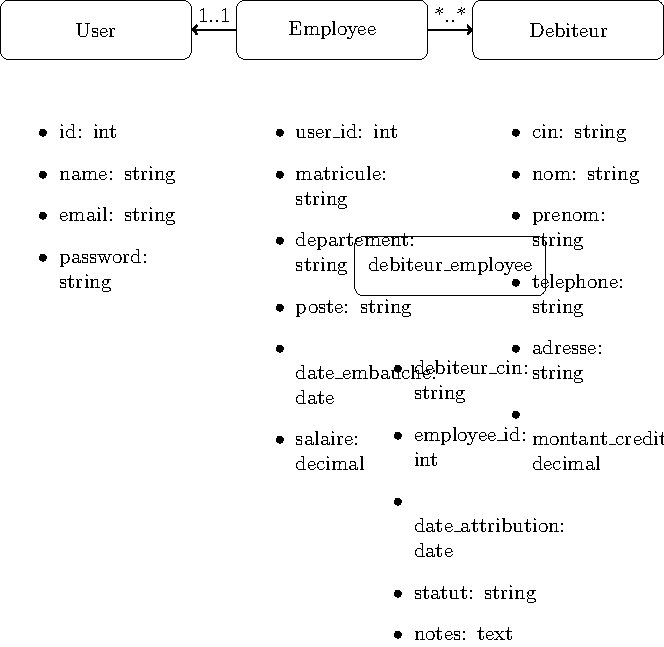
\includegraphics[width=\textwidth]{class_diagram.pdf}
    \caption{Diagramme de classes du système}
    \label{fig:class_diagram}
\end{figure}

Le diagramme de classes illustre la structure des données de notre application avec trois entités principales :
\begin{itemize}
    \item \textbf{User} : Gère l'authentification et les informations de base des utilisateurs
    \item \textbf{Employee} : Représente les employés avec leurs informations professionnelles
    \item \textbf{Debiteur} : Contient les informations des débiteurs et leurs montants de crédit
\end{itemize}

Les relations principales sont :
\begin{itemize}
    \item Une relation one-to-one entre Employee et User
    \item Une relation many-to-many entre Employee et Debiteur
    \item Une table pivot debiteur\_employee pour gérer les attributions
\end{itemize}

\subsection{Diagramme de Cas d'Utilisation}
\begin{figure}[H]
    \centering
    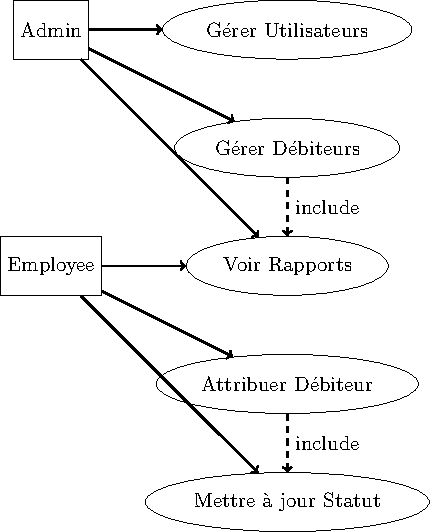
\includegraphics[width=\textwidth]{use_case_diagram.pdf}
    \caption{Diagramme de cas d'utilisation}
    \label{fig:use_case_diagram}
\end{figure}

Le diagramme de cas d'utilisation présente les principales fonctionnalités du système :
\begin{itemize}
    \item \textbf{Admin} : Gestion complète des utilisateurs et des débiteurs
    \item \textbf{Employee} : Attribution et suivi des débiteurs
    \item Fonctionnalités communes : Consultation des rapports
\end{itemize}

\subsection{Diagramme de Séquence}
\begin{figure}[H]
    \centering
    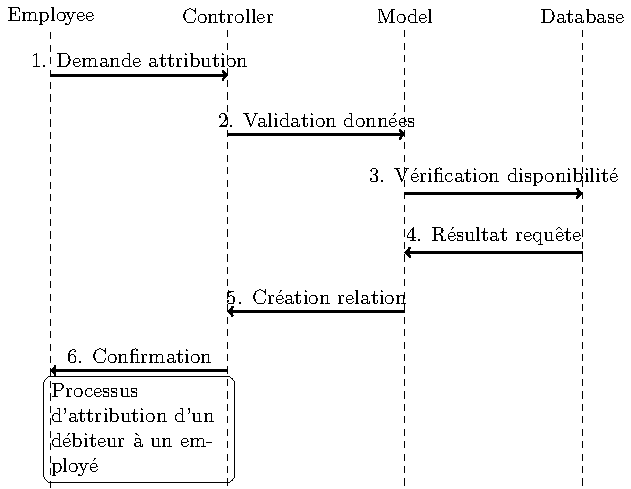
\includegraphics[width=\textwidth]{sequence_diagram.pdf}
    \caption{Diagramme de séquence - Processus d'attribution}
    \label{fig:sequence_diagram}
\end{figure}

Le diagramme de séquence illustre le processus d'attribution d'un débiteur :
\begin{enumerate}
    \item L'employé initie la demande d'attribution
    \item Le contrôleur valide les données
    \item Le modèle vérifie la disponibilité
    \item La base de données est consultée
    \item La relation est créée
    \item Une confirmation est envoyée
\end{enumerate}

\subsection{Diagramme d'Activité}
\begin{figure}[H]
    \centering
    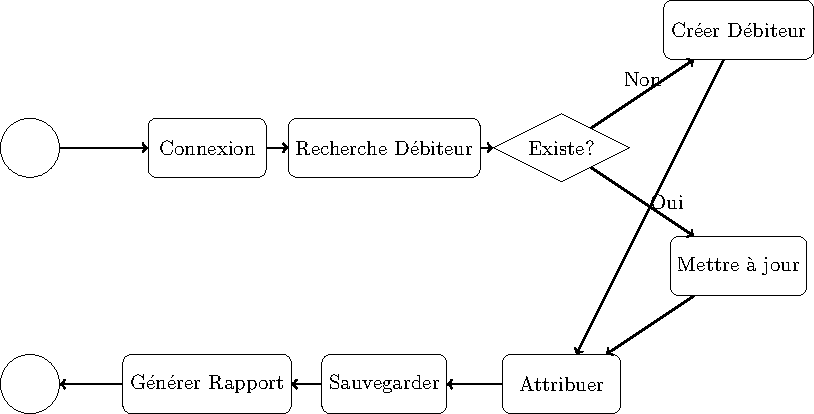
\includegraphics[width=\textwidth]{activity_diagram.pdf}
    \caption{Diagramme d'activité - Gestion des débiteurs}
    \label{fig:activity_diagram}
\end{figure}

Le diagramme d'activité montre le flux de travail complet pour la gestion des débiteurs :
\begin{itemize}
    \item Processus de connexion
    \item Recherche de débiteur
    \item Création ou mise à jour
    \item Attribution
    \item Génération de rapports
\end{itemize}

\subsection{Diagramme de Déploiement}
\begin{figure}[H]
    \centering
    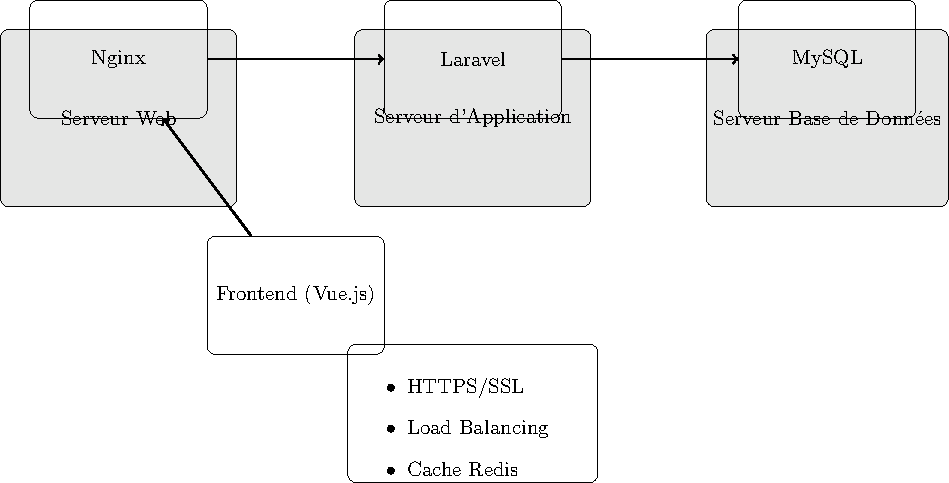
\includegraphics[width=\textwidth]{deployment_diagram.pdf}
    \caption{Diagramme de déploiement de l'application}
    \label{fig:deployment_diagram}
\end{figure}

L'architecture de déploiement comprend :
\begin{itemize}
    \item \textbf{Serveur Web} : Nginx pour la gestion des requêtes
    \item \textbf{Serveur d'Application} : Laravel pour la logique métier
    \item \textbf{Base de Données} : MySQL pour le stockage
    \item \textbf{Frontend} : Application Vue.js
\end{itemize}

\subsection{Diagramme de Composants}
\begin{figure}[H]
    \centering
    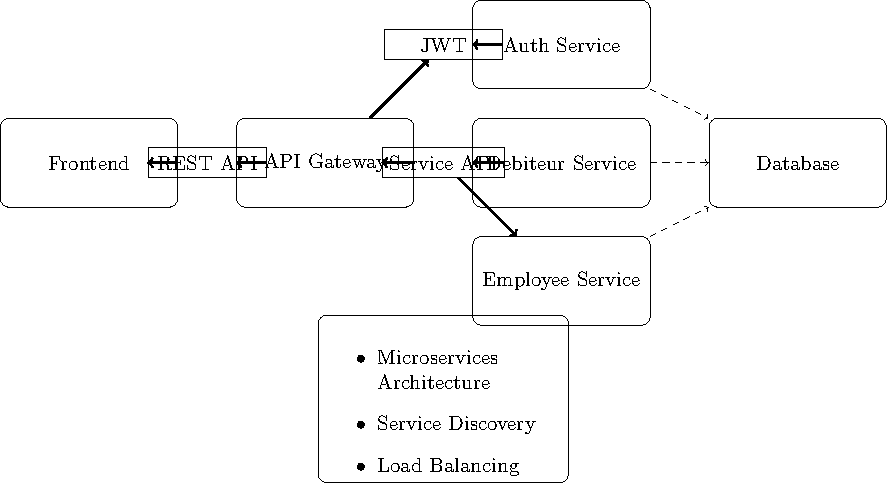
\includegraphics[width=\textwidth]{component_diagram.pdf}
    \caption{Diagramme de composants de l'application}
    \label{fig:component_diagram}
\end{figure}

L'architecture des composants montre :
\begin{itemize}
    \item \textbf{Frontend} : Interface utilisateur
    \item \textbf{API Gateway} : Point d'entrée unique
    \item \textbf{Services} : Auth, Debiteur, Employee
    \item \textbf{Base de données} : Stockage centralisé
\end{itemize}

% Chapitre 3: Réalisation
\chapter{Réalisation}
\section{Environnement de Développement}
\begin{itemize}
    \item Backend: Laravel 10.x
    \item Frontend: JavaScript/TypeScript avec Tailwind CSS
    \item Base de données: MySQL 8.0
    \item Serveur web: Apache/Nginx
    \item Outils de développement:
        \begin{itemize}
            \item Git pour le contrôle de version
            \item Composer pour la gestion des dépendances PHP
            \item npm pour la gestion des dépendances JavaScript
            \item VS Code comme IDE principal
        \end{itemize}
\end{itemize}

\section{Structure du Code}
\subsection{Organisation du Backend}
\begin{itemize}
    \item \textbf{Models/}: Contient les modèles de données
    \item \textbf{Http/Controllers/}: Gestion des requêtes
    \item \textbf{Http/Middleware/}: Middleware d'authentification
    \item \textbf{Database/Migrations/}: Structure de la base de données
    \item \textbf{Routes/}: Définition des routes API
\end{itemize}

\subsection{Organisation du Frontend}
\begin{itemize}
    \item \textbf{src/components/}: Composants réutilisables
    \item \textbf{src/pages/}: Pages principales
    \item \textbf{src/services/}: Services API
    \item \textbf{src/store/}: Gestion d'état
\end{itemize}

\section{Fonctionnalités Implémentées}
\subsection{Gestion des Débiteurs}
\begin{itemize}
    \item Création et modification des profils débiteurs
    \item Suivi des montants de crédit
    \item Historique des transactions
    \item Recherche et filtrage avancés
\end{itemize}

\subsection{Gestion des Employés}
\begin{itemize}
    \item Gestion des profils employés
    \item Attribution des débiteurs
    \item Suivi des performances
    \item Gestion des permissions
\end{itemize}

\subsection{Rapports et Statistiques}
\begin{itemize}
    \item Tableaux de bord personnalisés
    \item Rapports exportables
    \item Visualisations graphiques
    \item Métriques de performance
\end{itemize}

% Chapitre 4: Tests et Validation
\chapter{Tests et Validation}
\section{Stratégie de Test}
\subsection{Tests Unitaires}
\begin{itemize}
    \item Tests des modèles
    \item Tests des contrôleurs
    \item Tests des services
\end{itemize}

\subsection{Tests d'Intégration}
\begin{itemize}
    \item Tests des API
    \item Tests des relations entre modèles
    \item Tests de validation des données
\end{itemize}

\subsection{Tests de Performance}
\begin{itemize}
    \item Tests de charge
    \item Tests de temps de réponse
    \item Tests d'optimisation
\end{itemize}

\section{Résultats des Tests}
[Présentation des résultats]

% Chapitre 5: Déploiement
\chapter{Déploiement}
\section{Environnement de Production}
[Description de l'environnement de production]

\section{Procédure de Déploiement}
[Description des étapes de déploiement]

% Conclusion
\chapter{Conclusion}
\section{Bilan du Projet}
Le projet de Système de Gestion des Débiteurs a été réalisé avec succès, répondant aux objectifs initiaux tout en respectant les contraintes techniques et fonctionnelles. Les principales réalisations incluent :

\begin{itemize}
    \item Une architecture robuste et évolutive
    \item Une interface utilisateur intuitive
    \item Un système de gestion des débiteurs complet
    \item Une base de données optimisée
    \item Des fonctionnalités de reporting avancées
\end{itemize}

\section{Perspectives}
Les perspectives d'évolution du projet incluent :

\begin{itemize}
    \item Intégration de fonctionnalités de paiement en ligne
    \item Développement d'une application mobile
    \item Ajout de fonctionnalités d'intelligence artificielle
    \item Amélioration des capacités de reporting
    \item Intégration avec d'autres systèmes
\end{itemize}

% Bibliographie
\chapter{Bibliographie}
\begin{thebibliography}{9}
    \bibitem{laravel} Laravel Documentation, \url{https://laravel.com/docs}
    \bibitem{tailwind} Tailwind CSS Documentation, \url{https://tailwindcss.com/docs}
\end{thebibliography}

% Annexes
\appendix
\chapter{Annexes}
\section{Diagrammes UML}
\subsection{Diagramme de Classes}
\begin{figure}[H]
    \centering
    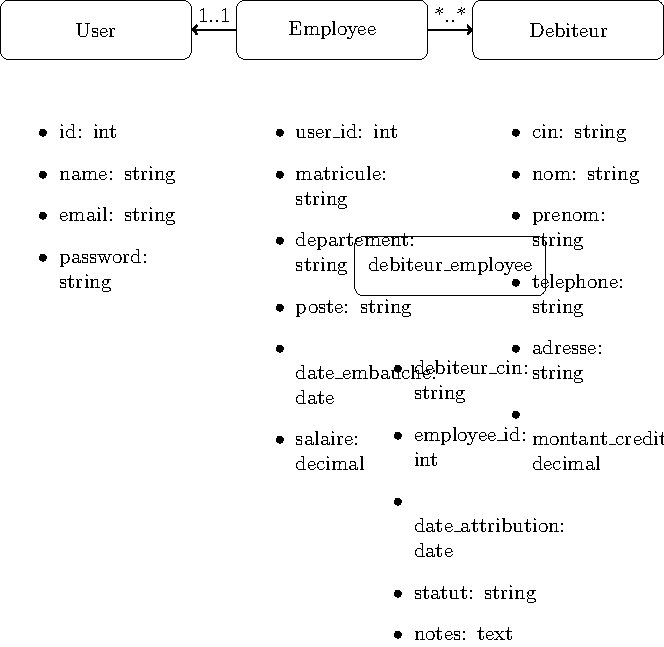
\includegraphics[width=\textwidth]{class_diagram.pdf}
    \caption{Diagramme de classes du système}
    \label{fig:class_diagram}
\end{figure}

\subsection{Diagramme de Cas d'Utilisation}
\begin{figure}[H]
    \centering
    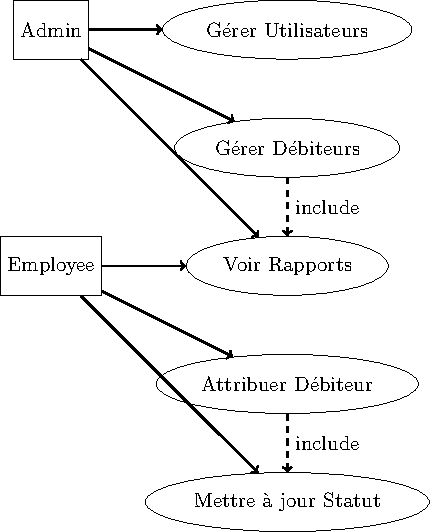
\includegraphics[width=\textwidth]{use_case_diagram.pdf}
    \caption{Diagramme de cas d'utilisation}
    \label{fig:use_case_diagram}
\end{figure}

\subsection{Diagramme de Séquence}
\begin{figure}[H]
    \centering
    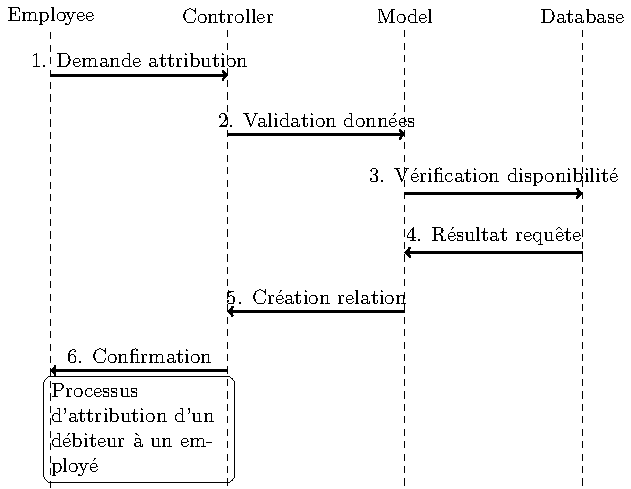
\includegraphics[width=\textwidth]{sequence_diagram.pdf}
    \caption{Diagramme de séquence - Processus d'attribution}
    \label{fig:sequence_diagram}
\end{figure}

\subsection{Diagramme d'Activité}
\begin{figure}[H]
    \centering
    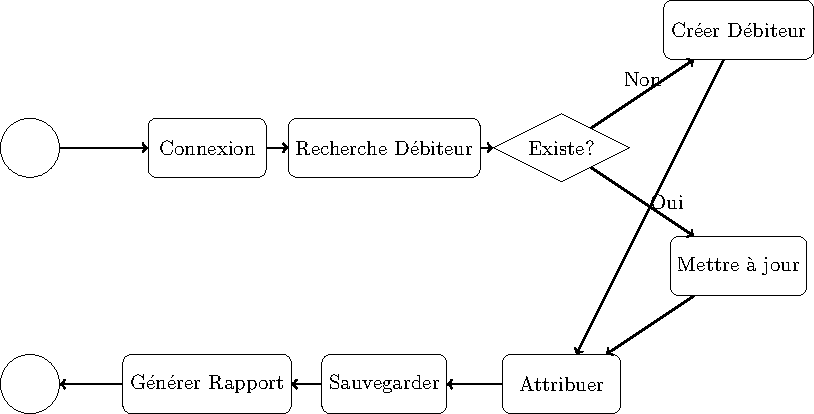
\includegraphics[width=\textwidth]{activity_diagram.pdf}
    \caption{Diagramme d'activité - Gestion des débiteurs}
    \label{fig:activity_diagram}
\end{figure}

\subsection{Diagramme de Déploiement}
\begin{figure}[H]
    \centering
    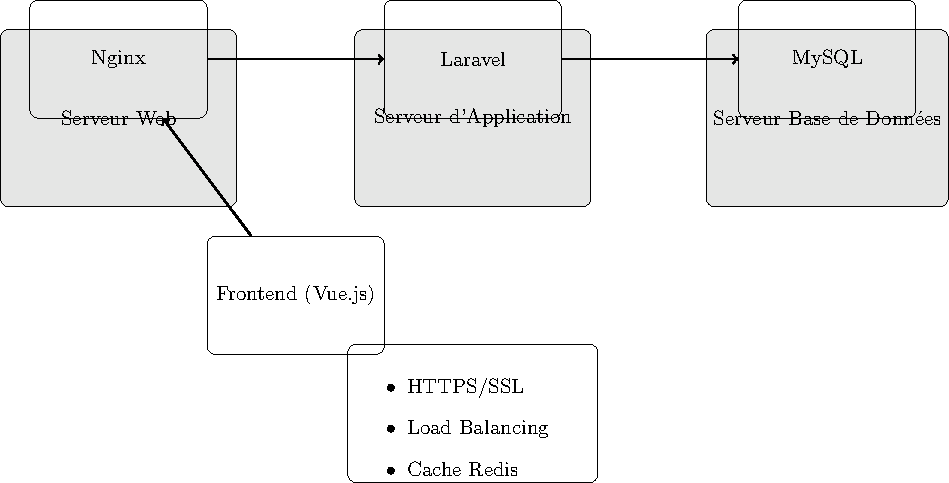
\includegraphics[width=\textwidth]{deployment_diagram.pdf}
    \caption{Diagramme de déploiement de l'application}
    \label{fig:deployment_diagram}
\end{figure}

\subsection{Diagramme de Composants}
\begin{figure}[H]
    \centering
    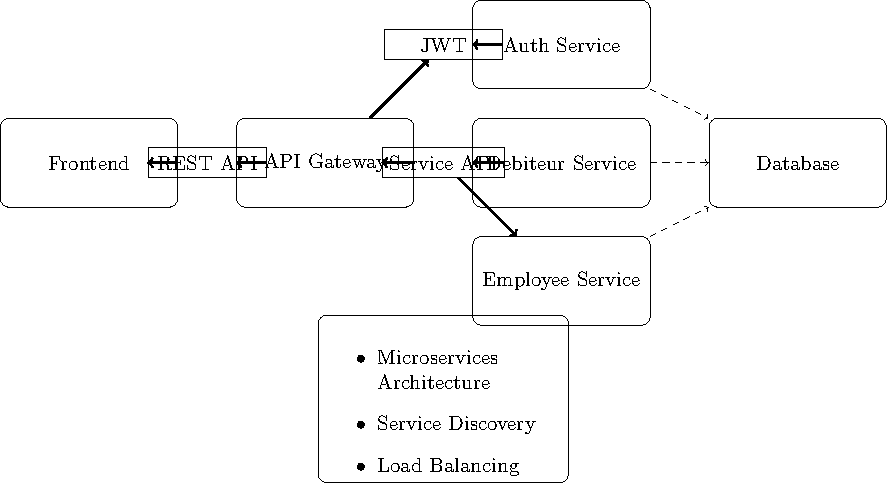
\includegraphics[width=\textwidth]{component_diagram.pdf}
    \caption{Diagramme de composants de l'application}
    \label{fig:component_diagram}
\end{figure}

\section{Manuel d'Utilisation}
[Documentation utilisateur]

\section{Code Source}
\subsection{Modèles}
\subsubsection{Modèle Debiteur}
\begin{lstlisting}[language=PHP]
<?php

namespace App\Models;

use Illuminate\Database\Eloquent\Factories\HasFactory;
use Illuminate\Database\Eloquent\Model;

class Debiteur extends Model
{
    use HasFactory;

    protected $fillable = [
        'cin',
        'nom',
        'prenom',
        'telephone',
        'adresse',
        'montant_credit'
    ];

    protected $primaryKey = 'cin';
    public $incrementing = false;
    protected $keyType = 'string';

    protected $casts = [
        'montant_credit' => 'decimal:2'
    ];

    public function employees()
    {
        return $this->belongsToMany(Employee::class, 'debiteur_employee', 
            'debiteur_cin', 'employee_id')
            ->withPivot(['date_attribution', 'statut', 'notes'])
            ->withTimestamps();
    }
}
\end{lstlisting}

\subsubsection{Modèle Employee}
\begin{lstlisting}[language=PHP]
<?php

namespace App\Models;

use Illuminate\Database\Eloquent\Factories\HasFactory;
use Illuminate\Database\Eloquent\Model;

class Employee extends Model
{
    use HasFactory;

    protected $fillable = [
        'user_id',
        'matricule',
        'departement',
        'poste',
        'date_embauche',
        'salaire',
        'telephone',
        'adresse'
    ];

    protected $casts = [
        'date_embauche' => 'date',
        'salaire' => 'decimal:2'
    ];

    public function user()
    {
        return $this->belongsTo(User::class);
    }

    public function debiteurs()
    {
        return $this->belongsToMany(Debiteur::class, 'debiteur_employee', 
            'employee_id', 'debiteur_cin')
            ->withPivot(['date_attribution', 'statut', 'notes'])
            ->withTimestamps();
    }
}
\end{lstlisting}

\subsection{Contrôleurs}
\subsubsection{DebiteurController}
\begin{lstlisting}[language=PHP]
<?php

namespace App\Http\Controllers;

use App\Models\Debiteur;
use Illuminate\Http\Request;

class DebiteurController extends Controller
{
    public function index()
    {
        $debiteurs = Debiteur::with('employees')->get();
        return response()->json($debiteurs);
    }

    public function store(Request $request)
    {
        $validated = $request->validate([
            'cin' => 'required|unique:debiteurs',
            'nom' => 'required',
            'prenom' => 'required',
            'telephone' => 'required',
            'adresse' => 'required',
            'montant_credit' => 'required|numeric'
        ]);

        $debiteur = Debiteur::create($validated);
        return response()->json($debiteur, 201);
    }

    public function show(Debiteur $debiteur)
    {
        return response()->json($debiteur->load('employees'));
    }

    public function update(Request $request, Debiteur $debiteur)
    {
        $validated = $request->validate([
            'nom' => 'required',
            'prenom' => 'required',
            'telephone' => 'required',
            'adresse' => 'required',
            'montant_credit' => 'required|numeric'
        ]);

        $debiteur->update($validated);
        return response()->json($debiteur);
    }

    public function destroy(Debiteur $debiteur)
    {
        $debiteur->delete();
        return response()->json(null, 204);
    }
}
\end{lstlisting}

\subsection{Frontend}
\subsubsection{Composant DebiteurList}
\begin{lstlisting}[language=JavaScript]
<template>
  <div class="debiteur-list">
    <h2>Liste des Débiteurs</h2>
    <div class="filters">
      <input v-model="search" placeholder="Rechercher...">
      <select v-model="filter">
        <option value="">Tous</option>
        <option value="actif">Actifs</option>
        <option value="inactif">Inactifs</option>
      </select>
    </div>
    
    <table>
      <thead>
        <tr>
          <th>CIN</th>
          <th>Nom</th>
          <th>Prénom</th>
          <th>Montant</th>
          <th>Actions</th>
        </tr>
      </thead>
      <tbody>
        <tr v-for="debiteur in filteredDebiteurs" :key="debiteur.cin">
          <td>{{ debiteur.cin }}</td>
          <td>{{ debiteur.nom }}</td>
          <td>{{ debiteur.prenom }}</td>
          <td>{{ formatMontant(debiteur.montant_credit) }}</td>
          <td>
            <button @click="editDebiteur(debiteur)">Modifier</button>
            <button @click="deleteDebiteur(debiteur)">Supprimer</button>
          </td>
        </tr>
      </tbody>
    </table>
  </div>
</template>

<script>
export default {
  data() {
    return {
      debiteurs: [],
      search: '',
      filter: ''
    }
  },
  computed: {
    filteredDebiteurs() {
      return this.debiteurs.filter(debiteur => {
        const matchesSearch = 
          debiteur.nom.toLowerCase().includes(this.search.toLowerCase()) ||
          debiteur.prenom.toLowerCase().includes(this.search.toLowerCase()) ||
          debiteur.cin.includes(this.search);
        
        if (!this.filter) return matchesSearch;
        return matchesSearch && debiteur.statut === this.filter;
      });
    }
  },
  methods: {
    formatMontant(montant) {
      return new Intl.NumberFormat('fr-MA', {
        style: 'currency',
        currency: 'MAD'
      }).format(montant);
    },
    async fetchDebiteurs() {
      try {
        const response = await this.$axios.get('/api/debiteurs');
        this.debiteurs = response.data;
      } catch (error) {
        console.error('Erreur lors du chargement des débiteurs:', error);
      }
    }
  },
  mounted() {
    this.fetchDebiteurs();
  }
}
</script>

<style scoped>
.debiteur-list {
  padding: 20px;
}

.filters {
  margin-bottom: 20px;
  display: flex;
  gap: 10px;
}

table {
  width: 100%;
  border-collapse: collapse;
}

th, td {
  padding: 10px;
  border: 1px solid #ddd;
  text-align: left;
}

th {
  background-color: #f5f5f5;
}

button {
  margin: 0 5px;
  padding: 5px 10px;
  border: none;
  border-radius: 4px;
  cursor: pointer;
}

button:first-child {
  background-color: #4CAF50;
  color: white;
}

button:last-child {
  background-color: #f44336;
  color: white;
}
</style>
\end{lstlisting}

\section{Base de Données}
\subsection{Migrations}
\begin{lstlisting}[language=PHP]
<?php

use Illuminate\Database\Migrations\Migration;
use Illuminate\Database\Schema\Blueprint;
use Illuminate\Support\Facades\Schema;

return new class extends Migration
{
    public function up()
    {
        Schema::create('debiteurs', function (Blueprint $table) {
            $table->string('cin')->primary();
            $table->string('nom');
            $table->string('prenom');
            $table->string('telephone');
            $table->text('adresse');
            $table->decimal('montant_credit', 10, 2);
            $table->timestamps();
        });

        Schema::create('employees', function (Blueprint $table) {
            $table->id();
            $table->foreignId('user_id')->constrained();
            $table->string('matricule')->unique();
            $table->string('departement');
            $table->string('poste');
            $table->date('date_embauche');
            $table->decimal('salaire', 10, 2);
            $table->string('telephone');
            $table->text('adresse');
            $table->timestamps();
        });

        Schema::create('debiteur_employee', function (Blueprint $table) {
            $table->string('debiteur_cin');
            $table->foreignId('employee_id');
            $table->date('date_attribution');
            $table->string('statut');
            $table->text('notes')->nullable();
            $table->timestamps();

            $table->foreign('debiteur_cin')
                  ->references('cin')
                  ->on('debiteurs')
                  ->onDelete('cascade');
            $table->foreign('employee_id')
                  ->references('id')
                  ->on('employees')
                  ->onDelete('cascade');
        });
    }

    public function down()
    {
        Schema::dropIfExists('debiteur_employee');
        Schema::dropIfExists('employees');
        Schema::dropIfExists('debiteurs');
    }
};
\end{lstlisting}

\end{document} 